\documentclass[11pt]{article}
\usepackage[margin=1in]{geometry}
\usepackage{graphicx}
\usepackage{booktabs}
\usepackage{float}
\usepackage{hyperref}
\usepackage{array}
\usepackage{caption}
\usepackage{longtable}
\usepackage{parskip}
\usepackage[T1]{fontenc}
\usepackage{lmodern}

\graphicspath{{../Data/}}
\hypersetup{
    colorlinks=true,
    linkcolor=black,
    urlcolor=blue,
    citecolor=black
}

\title{Powering a Mars Colony: Comparing Solar, Fission, and Fusion Across Colony Growth\\INDENG 290 Final Project Report}
\author{Vineet Reddy \and Samuel Heinz \and Nicholas Fitzpatrick}
\date{Spring 2026}

\begin{document}

\maketitle

\begin{abstract}
This project compares solar, fission, and several fusion concepts for a Mars colony power system. We study the problem from three angles: feasibility, cost, and reliability under dust storms. The main result is a staged power timeline rather than a single winning technology. For an early low population outpost, fission with solar support is the most credible path. As the colony grows, solar remains useful as supplemental generation but does not replace firm baseload power. At larger colony scales, fusion becomes worth serious consideration because the number of required fission units grows quickly and projected fusion cost improves with scale. The project repository, report source, and slide deck are available at \href{https://github.com/vineet-reddy/MarsColonyNuclearFusion}{\nolinkurl{github.com/vineet-reddy/MarsColonyNuclearFusion}}.
\end{abstract}

\section{Introduction}

Future Mars missions will need continuous electric power for life support, thermal control, oxygen production, water recycling, communications, and general habitat operations. That requirement becomes harder on Mars because solar input is weaker than on Earth, nights are long, and dust storms can sharply reduce available solar power. The project is therefore not only asking whether fusion can power a Mars colony. It is asking what power mix makes sense as the colony moves from a small outpost to a larger settlement. The project was built around three questions:

\begin{enumerate}
    \item How should the colony power mix change as population and demand grow.
    \item How strongly do dust storms affect power reliability.
    \item Which fusion concept looks most credible on paper.
\end{enumerate}

The final scope is narrower than the original proposal in one important way. Fusion is not placed inside the sol by sol reliability simulator (one Martian day at a time) because we did not have a defensible way to model operational availability for systems that do not yet exist. Instead, fusion is evaluated through resource classification and cost modeling, while the reliability work focuses on solar and fission.

\section{Input Data and Provenance}

The project uses seven input CSV files. Two are downloaded datasets and five are tables prepared by the team for the model. Most of the other CSV files in the \path{Data/} folder are generated outputs written by the code.

\begin{table}[H]
    \centering
    \small
    \caption{Input CSV files and where they came from.}
    \begin{tabular}{>{\raggedright\arraybackslash}p{1.55in}>{\raggedright\arraybackslash}p{2.05in}>{\raggedright\arraybackslash}p{2.35in}}
        \toprule
        File & Description & Source and status \\
        \midrule
        \path{MDAD.csv} & Mars dust storm observations used to sample storm timing and duration near Jezero. & Downloaded from the Mars Dust Activity Database public release \cite{mdad}. \\
        \path{nuclear_capacity_data_annual.csv} & Terrestrial nuclear capacity and generation data used as a benchmark for fission capacity factors. & Downloaded from U.S. Energy Information Administration Electric Power Annual Table 4.08.B \cite{eia}. \\
        \path{fusion_reactor_specs.csv} & Reactor level assumptions for the fusion concepts compared in the cost and feasibility models. & Team assembled table based on SPARC \cite{sparc}, Princeton Satellite Systems material on direct fusion drive \cite{pss}, and Avalanche Energy Orbitron material \cite{avalanche}. \\
        \path{technology_screening_inputs.csv} & Screening rubric inputs for TRL and Mars operating penalties used to compute the adapted McKelvey coordinates. & Team built assumption table used to make the deployability scoring reproducible rather than hand placed on the chart. \\
        \path{habitat_engineering_constants.csv} & Colony demand assumptions for life support, water, oxygen, lighting, communications, medical load, and thermal load. & Team built assumption table anchored to NASA Mars DRA 5.0 and MOXIE power related mission context \cite{dra,moxie}. \\
        \path{storage_specs.csv} & Battery and storage assumptions used to track how long the colony can ride through low generation periods. & Team built benchmark table for storage assumptions used in the class model. \\
        \path{dust_penalty_curve.csv} & Seasonal solar derating curve that reduces modeled solar output across the simulated Mars year. & Team built seasonal solar derating curve used in the Mars year simulation. \\
        \bottomrule
    \end{tabular}
\end{table}

This distinction matters. The two downloaded inputs are MDAD and the annual nuclear capacity table. The other five input files are modeling inputs prepared for the project. In particular, the dust penalty curve is a simplified approximation, not a direct rover solar radiation dataset.

\section{Methods}

\subsection{Feasibility and cost}

We use a McKelvey style chart as an adapted feasibility framework, not as a literal claim that each power option is a mineral reserve. In its classical form, a McKelvey chart is used in resource economics to classify resources by two questions: how certain we are that the resource exists, and whether it is commercially recoverable. The high certainty and high commerciality corner corresponds to reserves, while lower certainty or lower commerciality areas represent resources that are known, possible, or technically interesting but not yet economically usable.

For this project, the same two axis idea is useful because the power options differ along two similar dimensions. We adapt ``certainty of existence'' to mean confidence that the power system exists as a deployable engineering system, not confidence that sunlight, uranium, or fusion fuel exists. We adapt ``chance of commerciality'' to mean the chance that the system could plausibly operate as a practical Mars colony power source after considering maturity, reliability, capacity factor, launch mass, and Mars specific operating constraints. The category names on the chart should therefore be read as analogies: fission is treated like a proved reserve because compact fission power is the closest to deployable baseload technology; solar is treated as prospective because sunlight is certain but Mars operation is limited by night, dust, storms, and storage needs; fusion concepts are not treated as proved because the reactor concepts are promising but have not yet demonstrated the operating maturity needed for a Mars power system.

The chart coordinates are computed from a deterministic screening rubric rather than manually placed. The rubric uses four inputs for each power option \(i\):

\begin{itemize}
    \item \(\mathrm{TRL}_i\): technology readiness level, on the standard 1 to 9 scale where 9 is most mature.
    \item \(A_i\): capacity factor, meaning the fraction of the year the system is assumed to produce its rated average output in the cost model.
    \item \(M_i\): Mars operating score, a 0 to 1 project input that penalizes technologies for Mars specific barriers such as dust, night, storage dependence, or lack of demonstrated surface operation.
    \item \(\mathrm{LCOE}_i\): levelized cost of energy, meaning the average lifetime cost per kilowatt hour after capital cost, launch cost, operating cost, lifetime, and capacity factor are included.
\end{itemize}

Those inputs are converted into two normalized intermediate scores. \(T_i\) is the technology readiness score, and \(C_i\) is the cost score. The cost score gives the cheapest option a value of 1 and gives more expensive options smaller values:

\[
T_i = \frac{\mathrm{TRL}_i}{9}, \qquad
C_i = \min\left(1,\frac{\min_j \mathrm{LCOE}_j}{\mathrm{LCOE}_i}\right).
\]

The adapted deployability coordinate \(D_i\) is the x-axis value in the chart. It combines readiness, assumed operating availability, and Mars-specific operating difficulty:

\[
D_i = 0.60T_i + 0.25A_i + 0.15M_i,
\]

The adapted commercial operation coordinate \(P_i\) is the y-axis value. It is multiplied by \(D_i\) so that a system cannot score as highly commercial if it is not yet deployable:

\[
P_i = D_i(0.55A_i + 0.25M_i + 0.20C_i).
\]

The weights are class project modeling assumptions. They intentionally put the most weight on technology maturity and expected operating availability, while still allowing Mars penalties and modeled cost to affect placement. The dashed 0.5 lines are qualitative thresholds, not calibrated probabilities. Point size represents net electric power, so the figure separates the maturity question from the scale question. This is why fusion can appear large and attractive on power or cost while still remaining below the proved analogue region.

We also compute an all in levelized cost of energy, or LCOE. LCOE is the model's average cost of delivered electricity over the system lifetime, measured in dollars per kilowatt hour. The model includes Earth side capital cost, launch cost, operating cost, lifetime, and capacity factor. Launch cost is set to \$1{,}500 per kilogram in the base case.

\subsection{Reliability model}

The reliability model estimates how often a candidate colony power system can meet the colony's electricity demand without an energy shortfall. In this report, reliability means the fraction of simulated sols where available generation plus battery discharge is enough to serve the full daily load. The model simulates one Mars year, or 668 sols, for 6 person, 100 person, and 2{,}000 person colonies. Demand is built from habitat assumptions for plug loads, water recycling, oxygen production, lighting, communications, medical load, and thermal load.

The site assumption is Jezero crater, the Mars region used by the Perseverance rover mission. We use Jezero because it gives the dust storm sampling a concrete location instead of treating Mars dust as globally uniform. Storm sequences are drawn from the Jezero relevant subset of MDAD. Solar output is reduced by the seasonal dust penalty curve and then cut further during sampled storm periods. Fission is treated as a high availability baseload source, and the battery state of charge is tracked across the year.

\subsection{Forecast comparison}

The forecast comparison predicts the colony's daily electricity demand, not the weather and not reactor output. The input series is the synthetic sol by sol demand curve generated from the habitat load model for each colony size. The project compares three simple demand forecast models: a constant mean baseline, a sinusoidal seasonal proxy labeled SARIMA, and a smoothed residual model labeled Transformer. This part of the project is a side analysis rather than the core result, but it gives one more check on how predictable the modeled colony load is across colony sizes.

\section{Results}

\subsection{Feasibility and cost}

The adapted McKelvey result is straightforward. Fission is the only option that lands in the high certainty and high commerciality corner. Solar is physically available but operationally limited on Mars, so it sits in a prospective category. CFS SPARC is Commonwealth Fusion Systems' proposed compact tokamak, a magnetic confinement fusion reactor concept used here as the large, high power fusion case. SPARC moves into the prospective analogue region because its projected power and cost are attractive, but its commercial operation score stays below the proved threshold because the technology is not yet deployable. The other fusion concepts remain contingent. This does not mean fusion fuel is scarce; it means the reactor technology is not yet a proved Mars power system.

\begin{table}[H]
    \centering
    \scriptsize
    \caption{Deterministic inputs and outputs for the adapted McKelvey screening rubric.}
    \begin{tabular}{>{\raggedright\arraybackslash}p{1.55in}rrrrrr>{\raggedright\arraybackslash}p{1.15in}}
        \toprule
        Source & TRL & Mars score & Capacity factor & LCOE & \(D_i\) & \(P_i\) & Category \\
        \midrule
        Solar PV & 9 & 0.55 & 0.25 & 7.61 & 0.745 & 0.217 & Prospective \\
        Fission, Kilopower class & 5 & 0.90 & 0.92 & 8.31 & 0.698 & 0.521 & Proved \\
        CFS SPARC & 4 & 0.35 & 0.80 & 0.64 & 0.519 & 0.378 & Prospective \\
        Princeton FRC & 3 & 0.30 & 0.75 & 2.16 & 0.432 & 0.236 & Contingent \\
        Avalanche Orbitron & 2 & 0.25 & 0.70 & 2.30 & 0.346 & 0.174 & Contingent \\
        \bottomrule
    \end{tabular}
\end{table}

\begin{figure}[H]
    \centering
    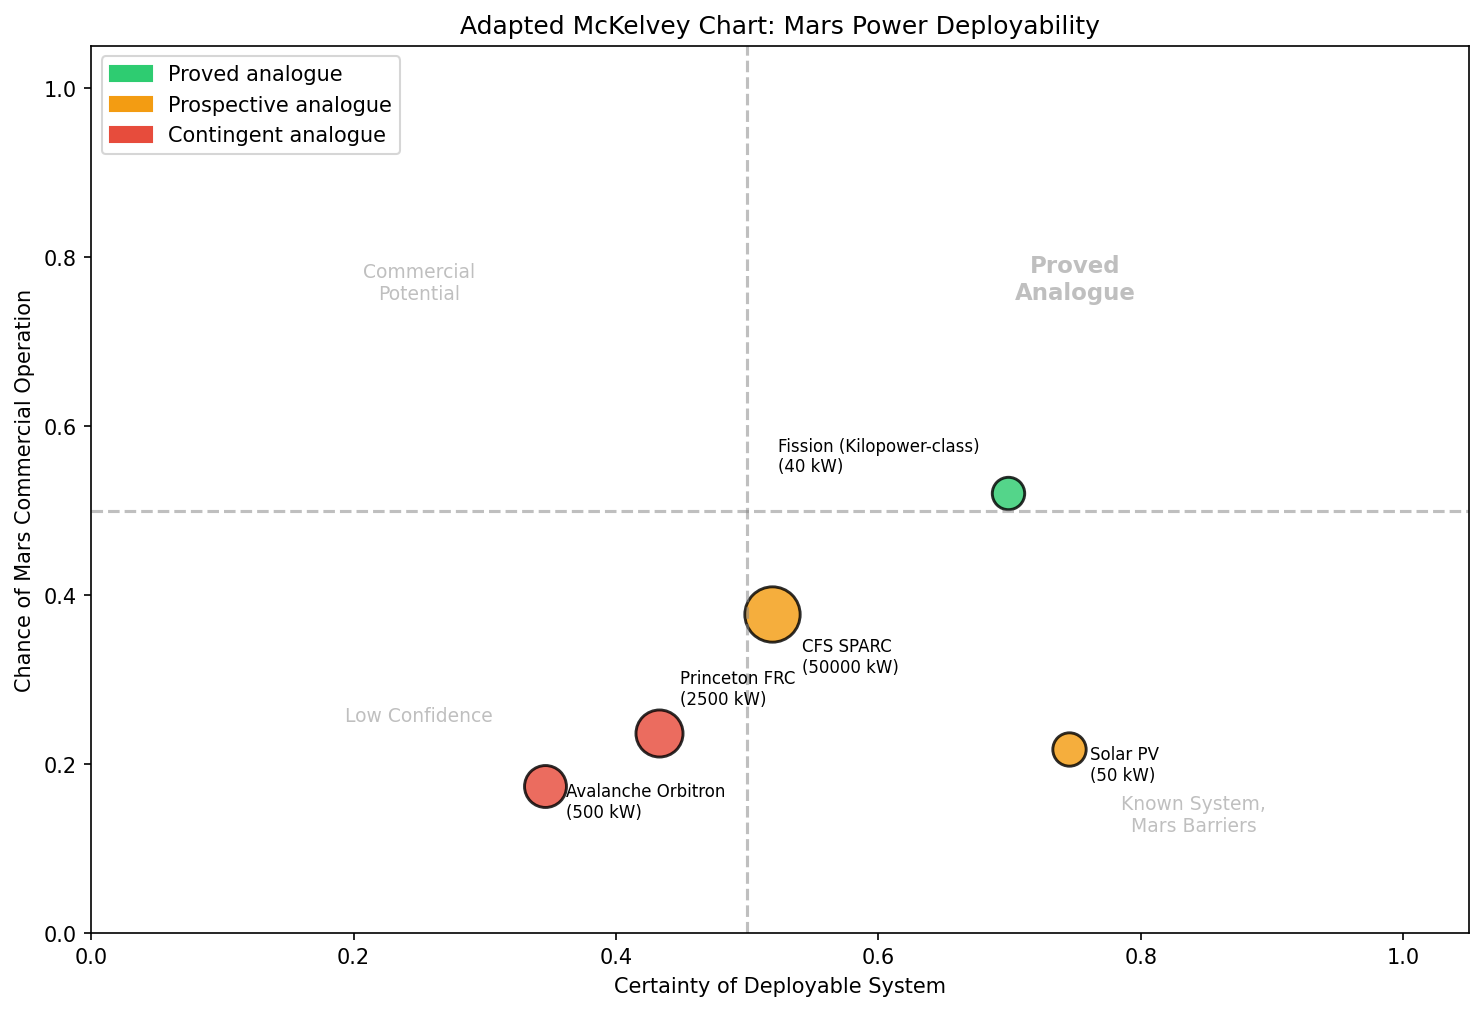
\includegraphics[width=0.82\textwidth]{mckelvey_box.png}
    \caption{Adapted McKelvey style deployability classification for the five power options. The axes borrow the structure of a classical resource chart but reinterpret it for power system maturity and Mars commercial practicality.}
\end{figure}

The cost model points in a different direction. On projected scale and cost, SPARC style fusion looks far cheaper than the other options. Solar and small fission units both remain expensive after launch is included.

\begin{table}[H]
    \centering
    \caption{Base LCOE results with launch cost included.}
    \label{tab:lcoe}
    \begin{tabular}{>{\raggedright\arraybackslash}p{2.7in}r}
        \toprule
        Source & LCOE (\$/kWh) \\
        \midrule
        Solar PV & 7.61 \\
        Fission, Kilopower class & 8.31 \\
        CFS SPARC & 0.64 \\
        Princeton FRC & 2.16 \\
        Avalanche Orbitron & 2.30 \\
        \bottomrule
    \end{tabular}
\end{table}

\begin{figure}[H]
    \centering
    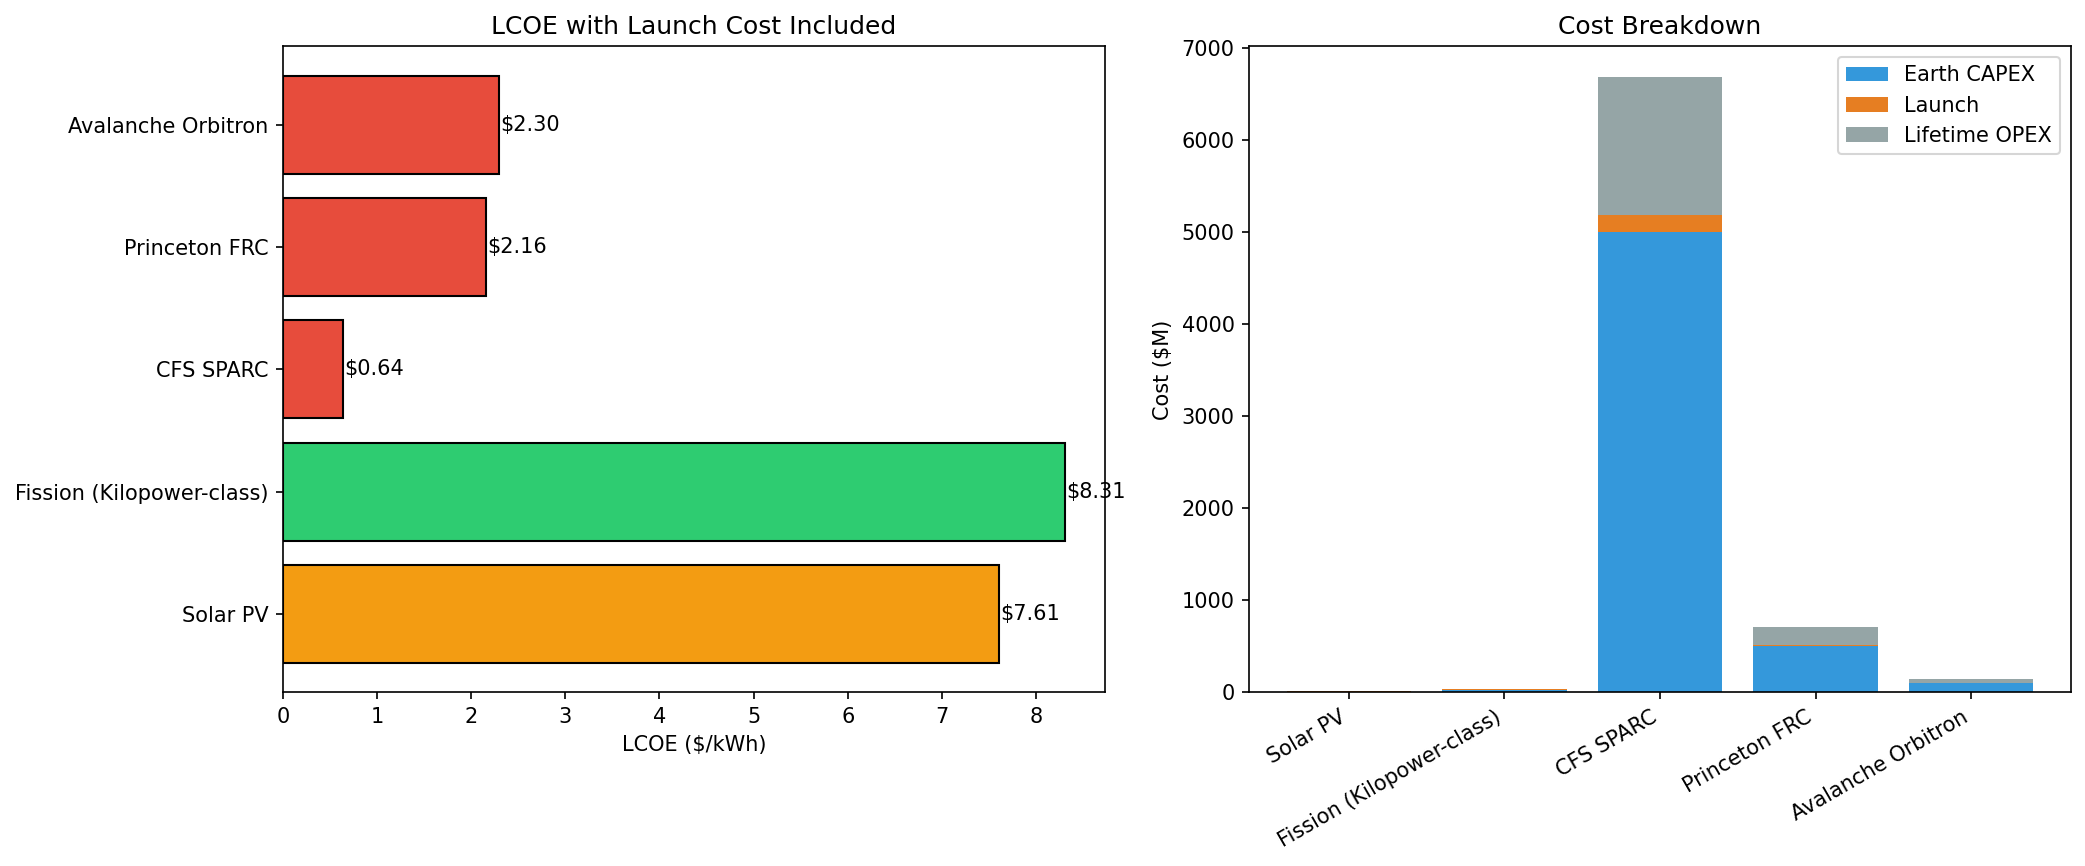
\includegraphics[width=\textwidth]{lcoe_comparison.png}
    \caption{All in cost comparison. The left panel shows LCOE and the right panel shows the cost breakdown.}
\end{figure}

Taken together, these two figures show the central tension in the project. Fission looks much more deployable now, but fusion looks stronger if the question is long run scale and projected cost.

\subsection{Reliability under dust storms}

The reliability results are much less ambiguous. The 6 person baseline case with solar plus fission is effectively perfect in the simulation, with a mean reliability of 1.0000 and a 5th percentile of 1.0000.

\begin{figure}[H]
    \centering
    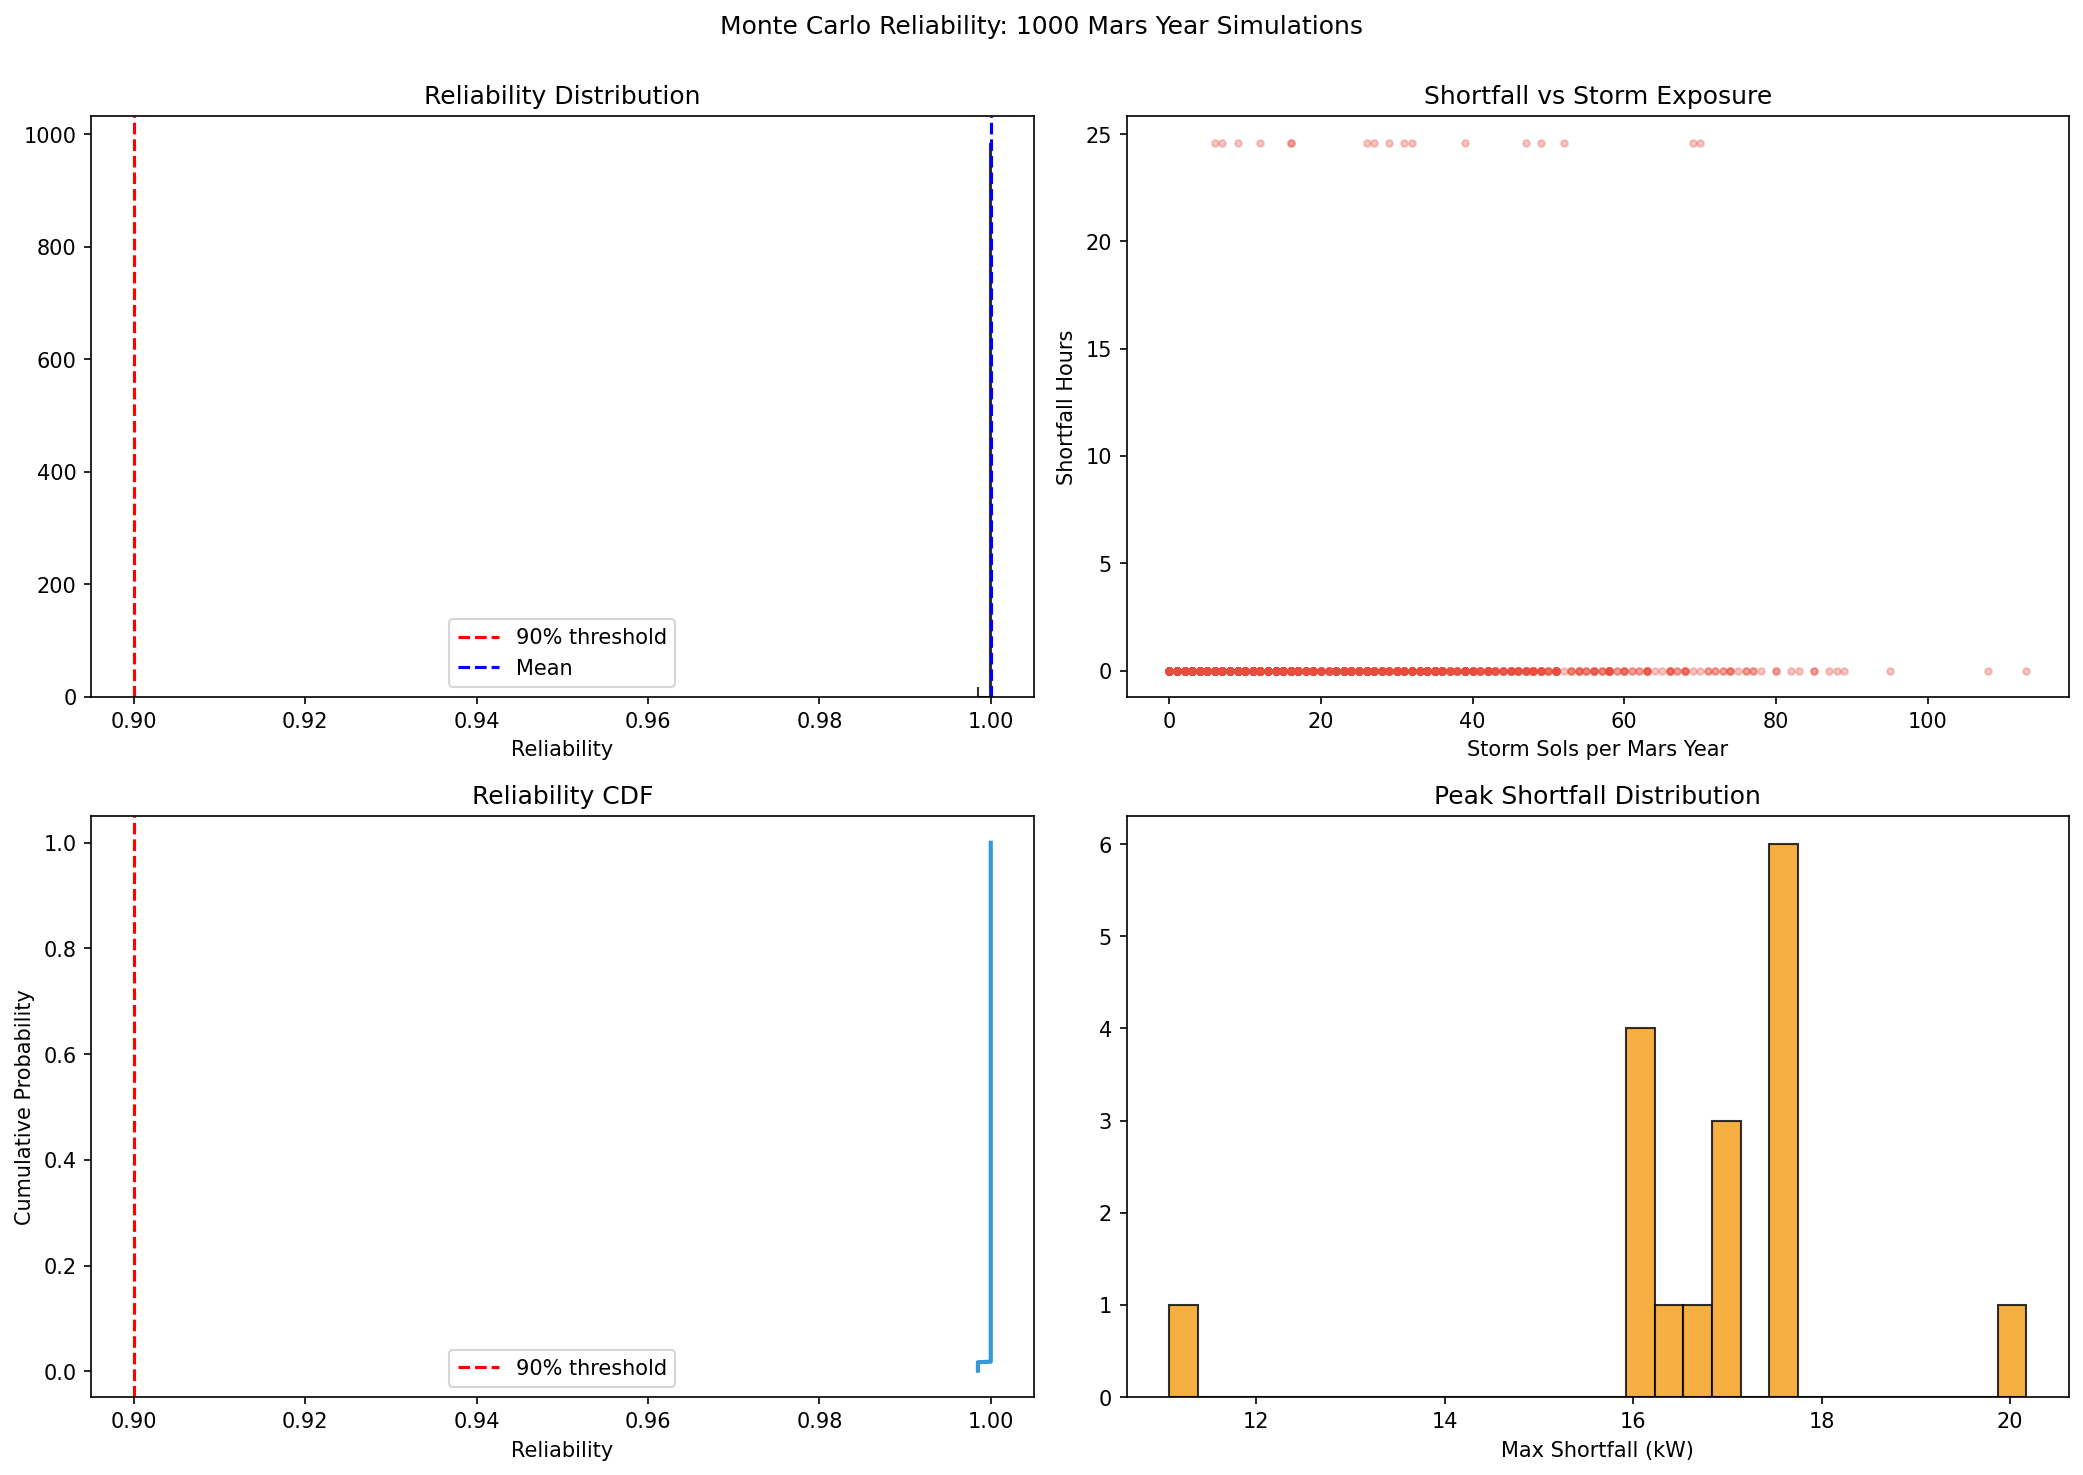
\includegraphics[width=\textwidth]{monte_carlo_reliability.png}
    \caption{Baseline Monte Carlo reliability for the 6 person solar plus fission case.}
\end{figure}

The scenario comparison is the clearest result in the report. Solar only systems perform poorly at every colony size we tested, while solar plus fission stays near full reliability.

\begin{table}[H]
    \centering
    \caption{Scenario reliability summary from the full simulation run.}
    \label{tab:scenarios}
    \begin{tabular}{>{\raggedright\arraybackslash}p{2.4in}rrr}
        \toprule
        Scenario & Mean reliability & 5th percentile & Zero shortfall share \\
        \midrule
        6p Solar only & 0.1379 & 0.1107 & 0.000 \\
        6p Solar plus Fission & 1.0000 & 1.0000 & 0.984 \\
        100p Solar only & 0.2123 & 0.1796 & 0.000 \\
        100p Solar plus Fission & 0.9960 & 0.9910 & 0.062 \\
        2000p Solar only & 0.2068 & 0.1751 & 0.000 \\
        2000p Solar plus Fission & 0.9958 & 0.9910 & 0.070 \\
        \bottomrule
    \end{tabular}
\end{table}

\begin{figure}[H]
    \centering
    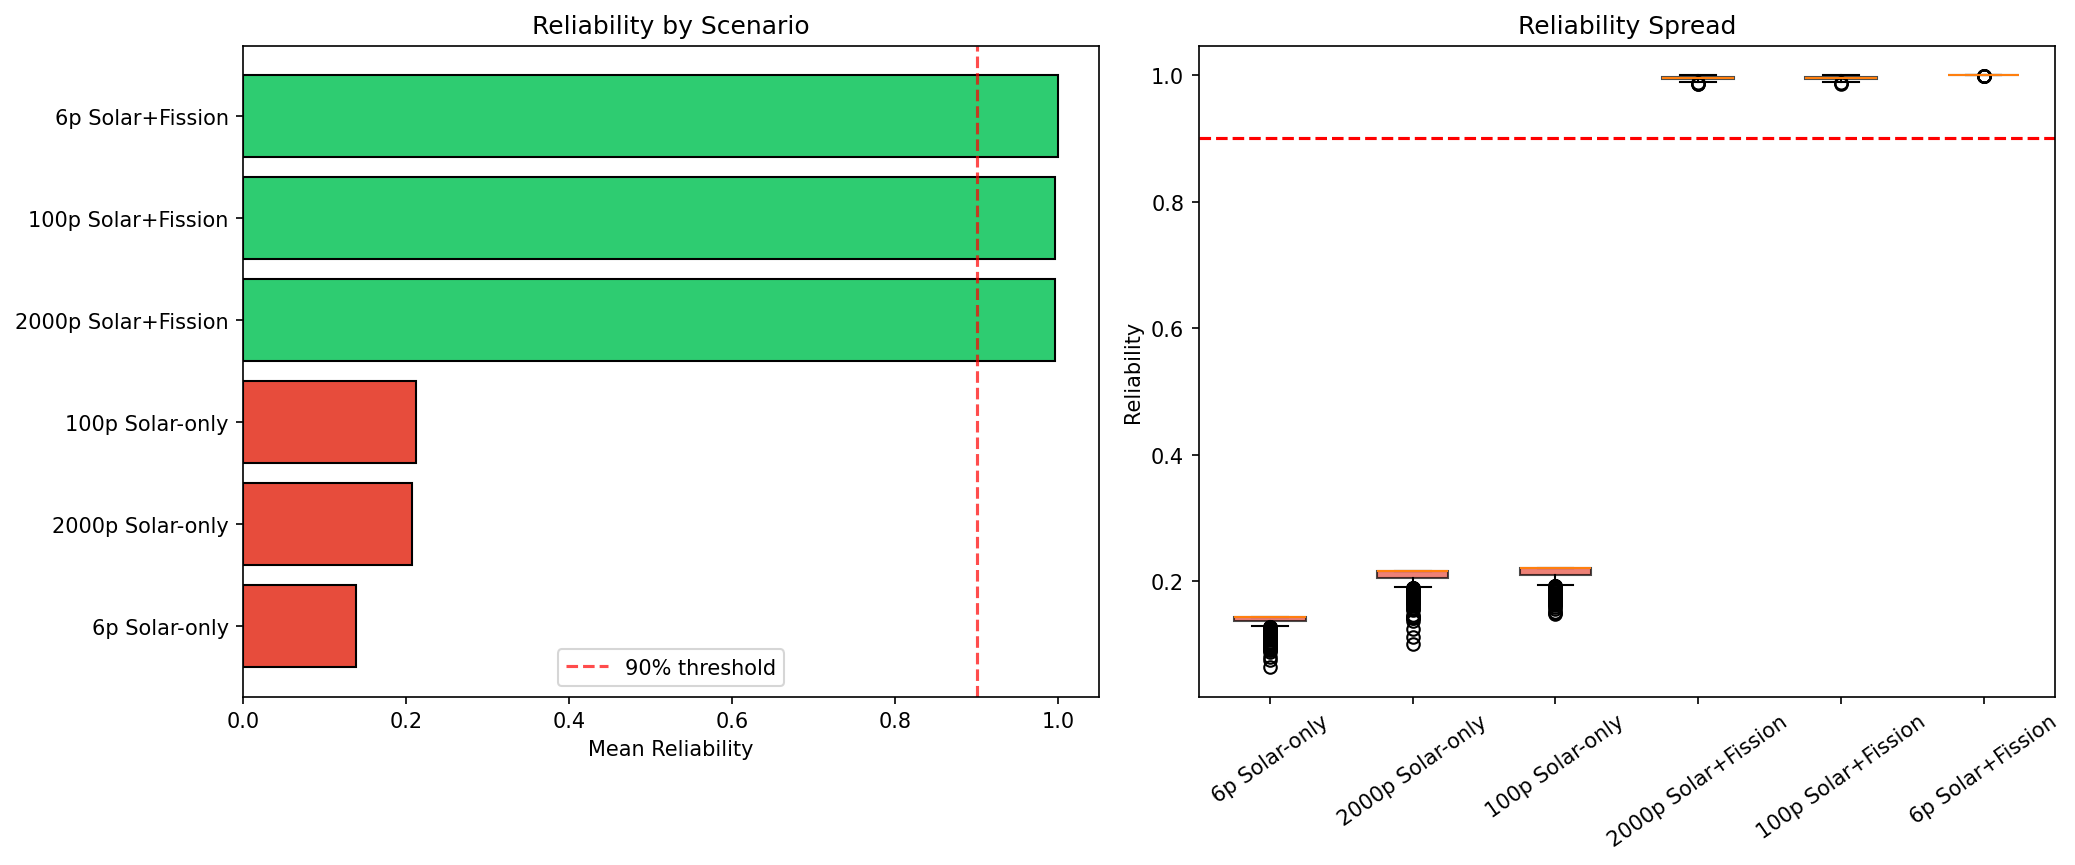
\includegraphics[width=\textwidth]{scenario_reliability.png}
    \caption{Reliability across colony size and supply mix.}
\end{figure}

\subsection{Scaling and sensitivity}

The scaling studies explain why fusion still matters in the project even though fission wins the near term reliability argument. For the 100 person colony, 8 Kilopower units are enough to cross 90 percent mean reliability. For the 2{,}000 person colony, the same threshold takes 160 units. That does not make large scale fission impossible, but it does show why the logistics become unattractive.

\begin{figure}[H]
    \centering
    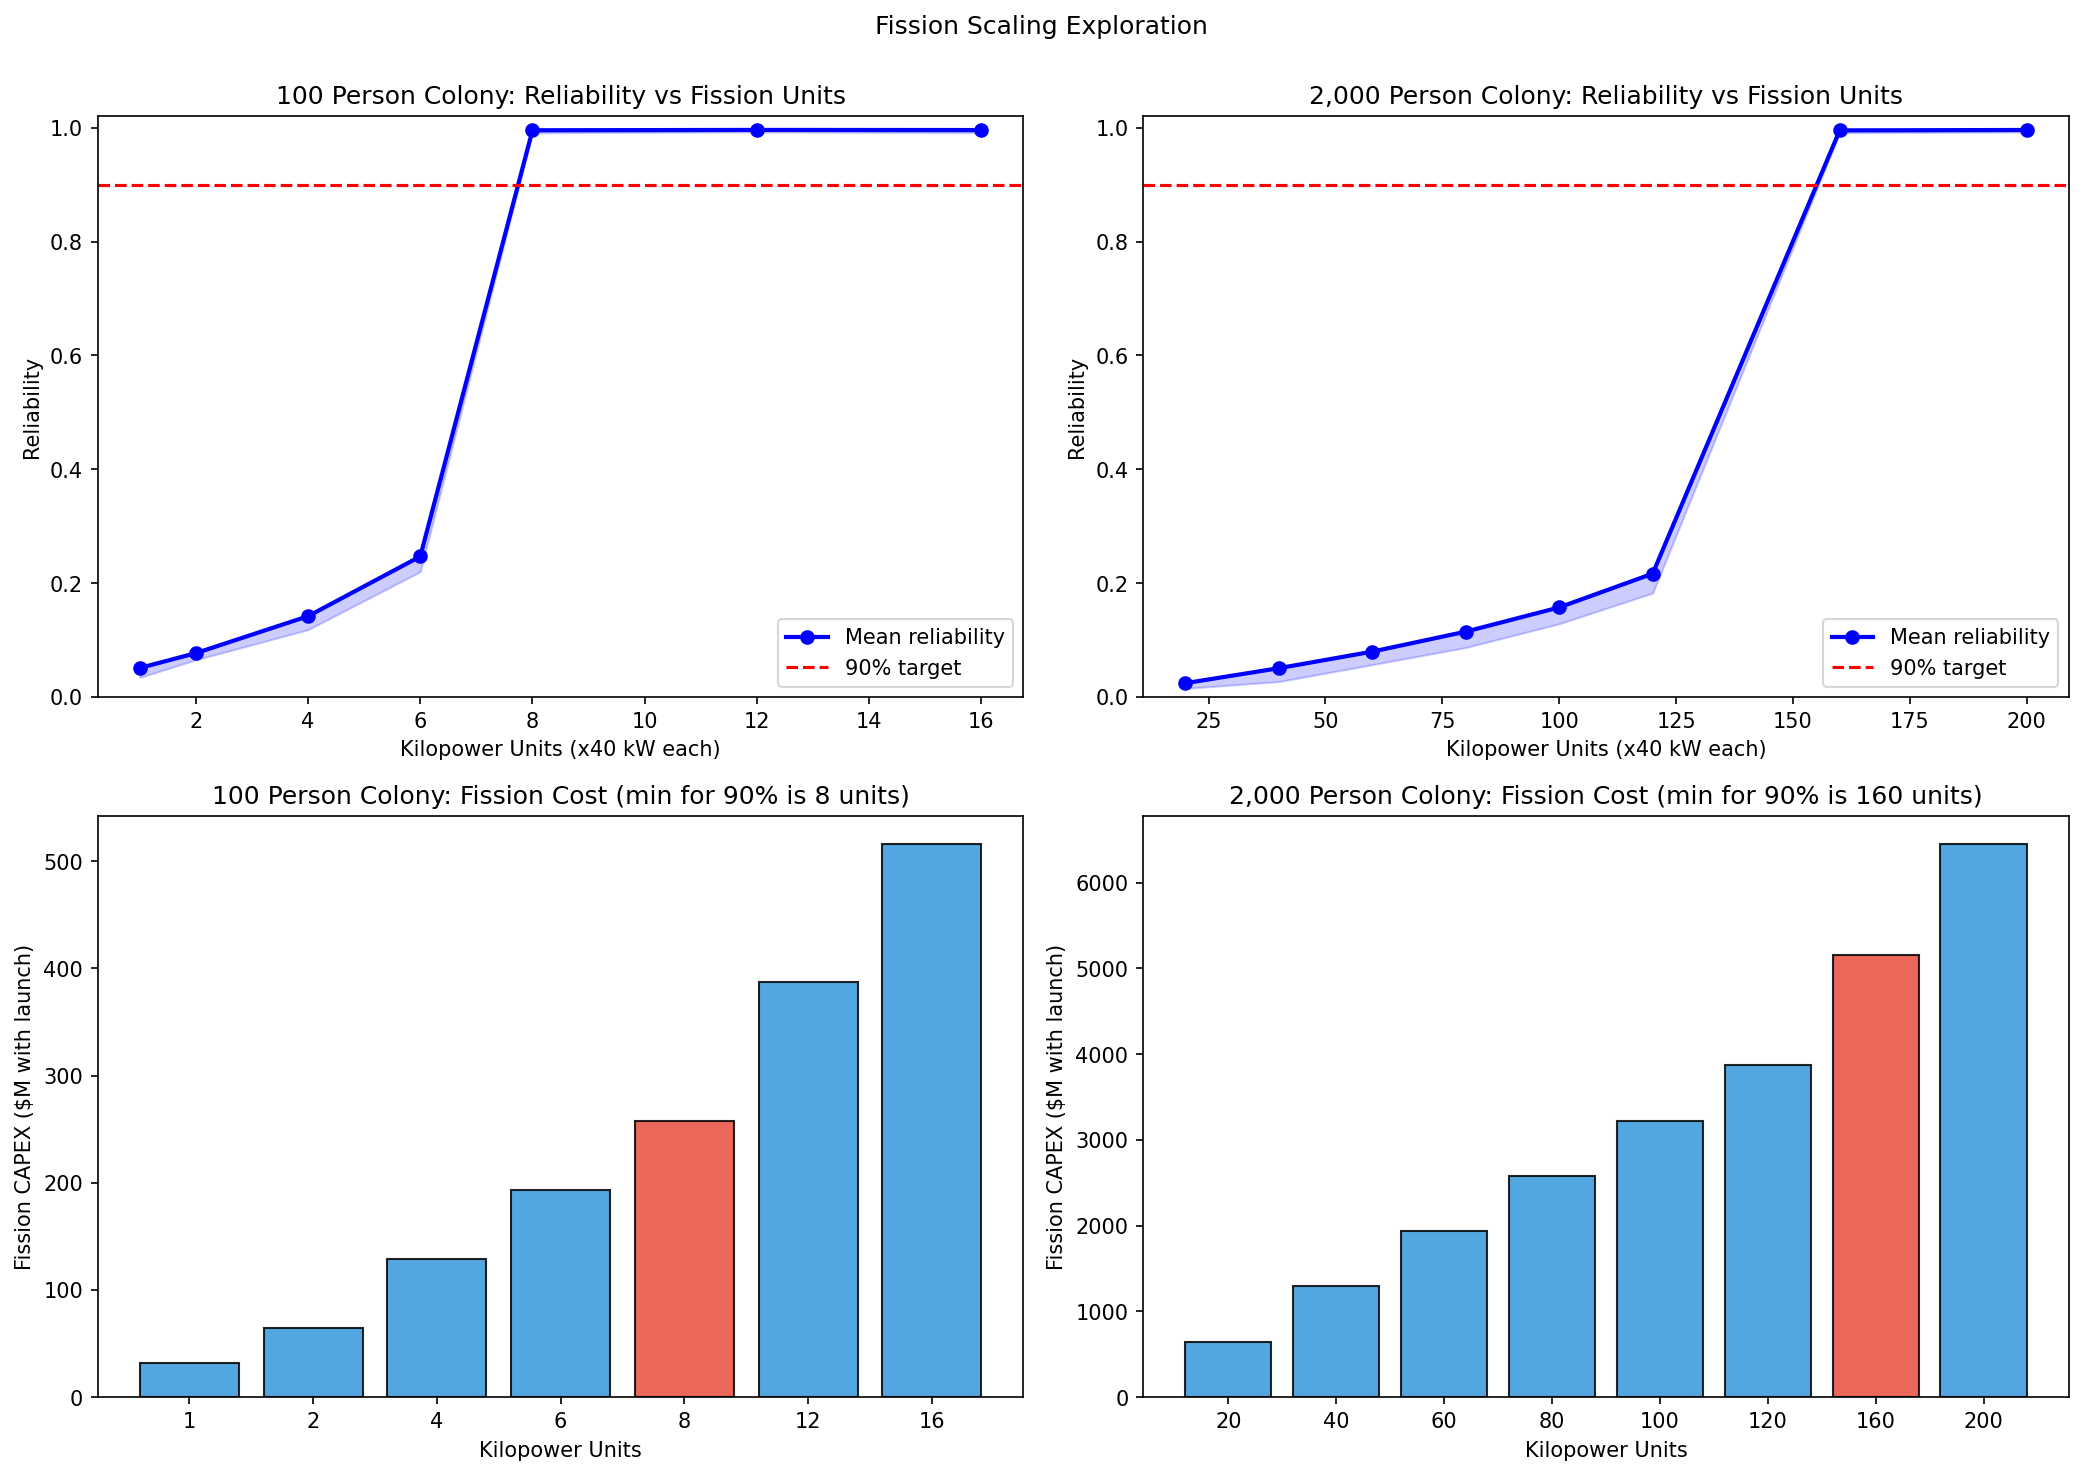
\includegraphics[width=\textwidth]{fission_scaling.png}
    \caption{Fission scaling for the 100 person and 2{,}000 person cases.}
\end{figure}

The sensitivity work does not overturn the basic story. The TRL mapping changes the exact fusion placement in the adapted McKelvey chart, and launch cost can move the ordering near the bottom of the LCOE ranking, but none of those changes make fusion mature today or make solar only systems reliable.

\begin{figure}[H]
    \centering
    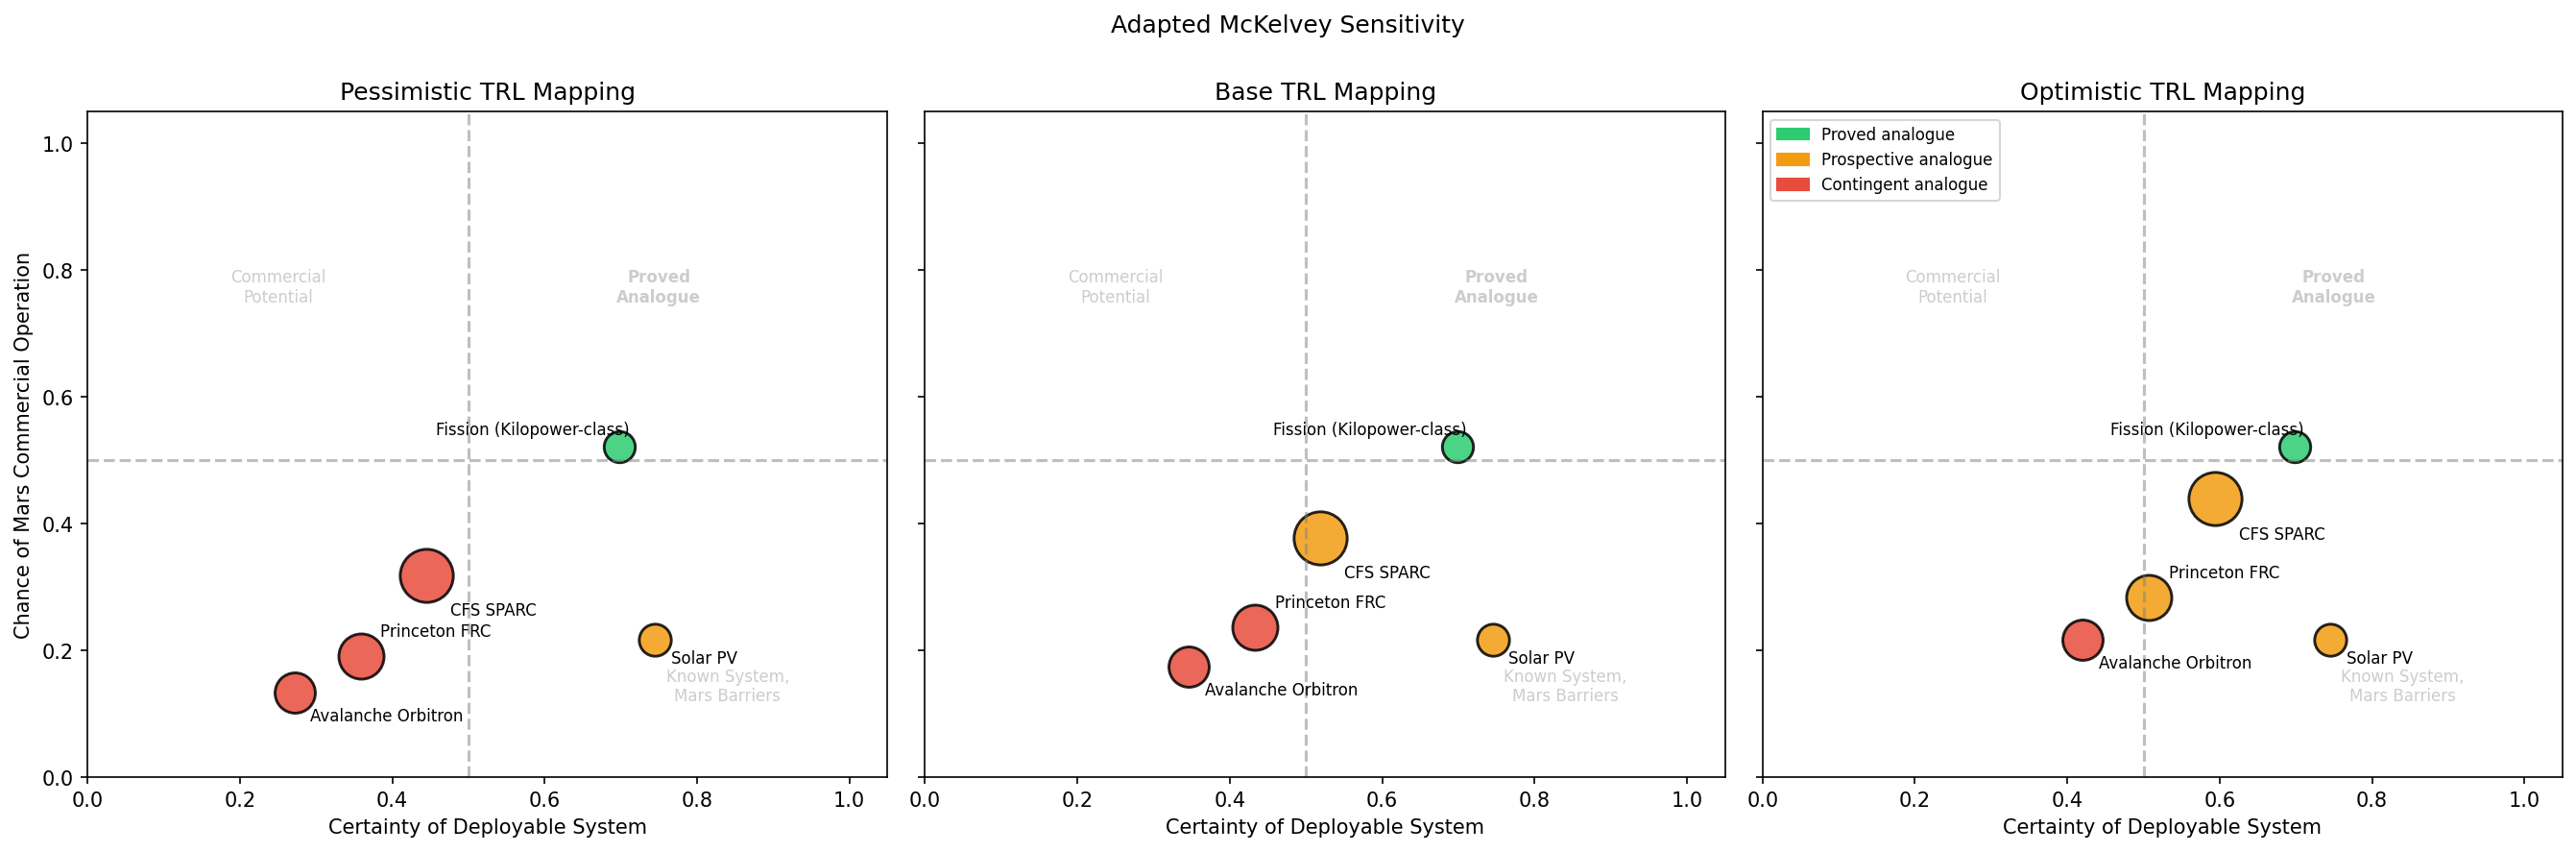
\includegraphics[width=\textwidth]{mckelvey_sensitivity.png}
    \caption{Adapted McKelvey sensitivity to different maturity assumptions.}
\end{figure}

\begin{figure}[H]
    \centering
    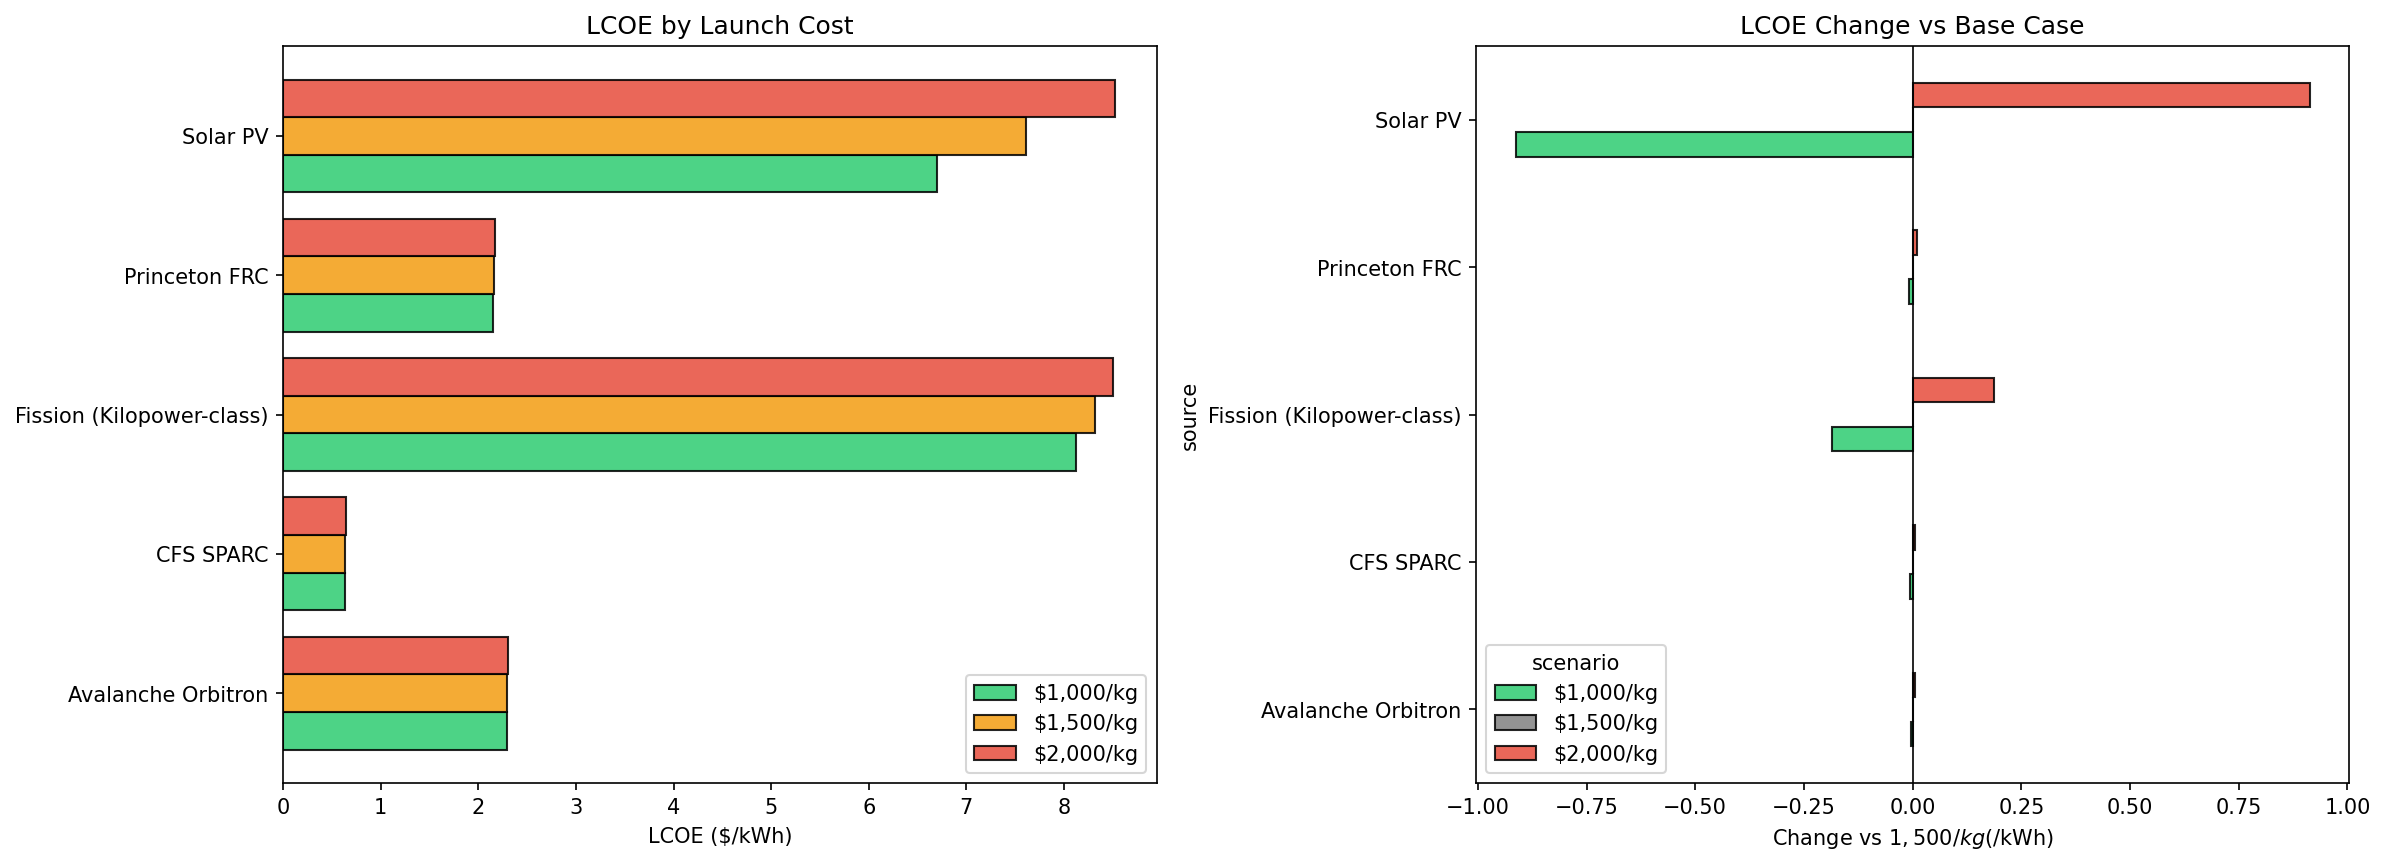
\includegraphics[width=\textwidth]{lcoe_sensitivity.png}
    \caption{LCOE sensitivity to launch cost.}
\end{figure}

\begin{figure}[H]
    \centering
    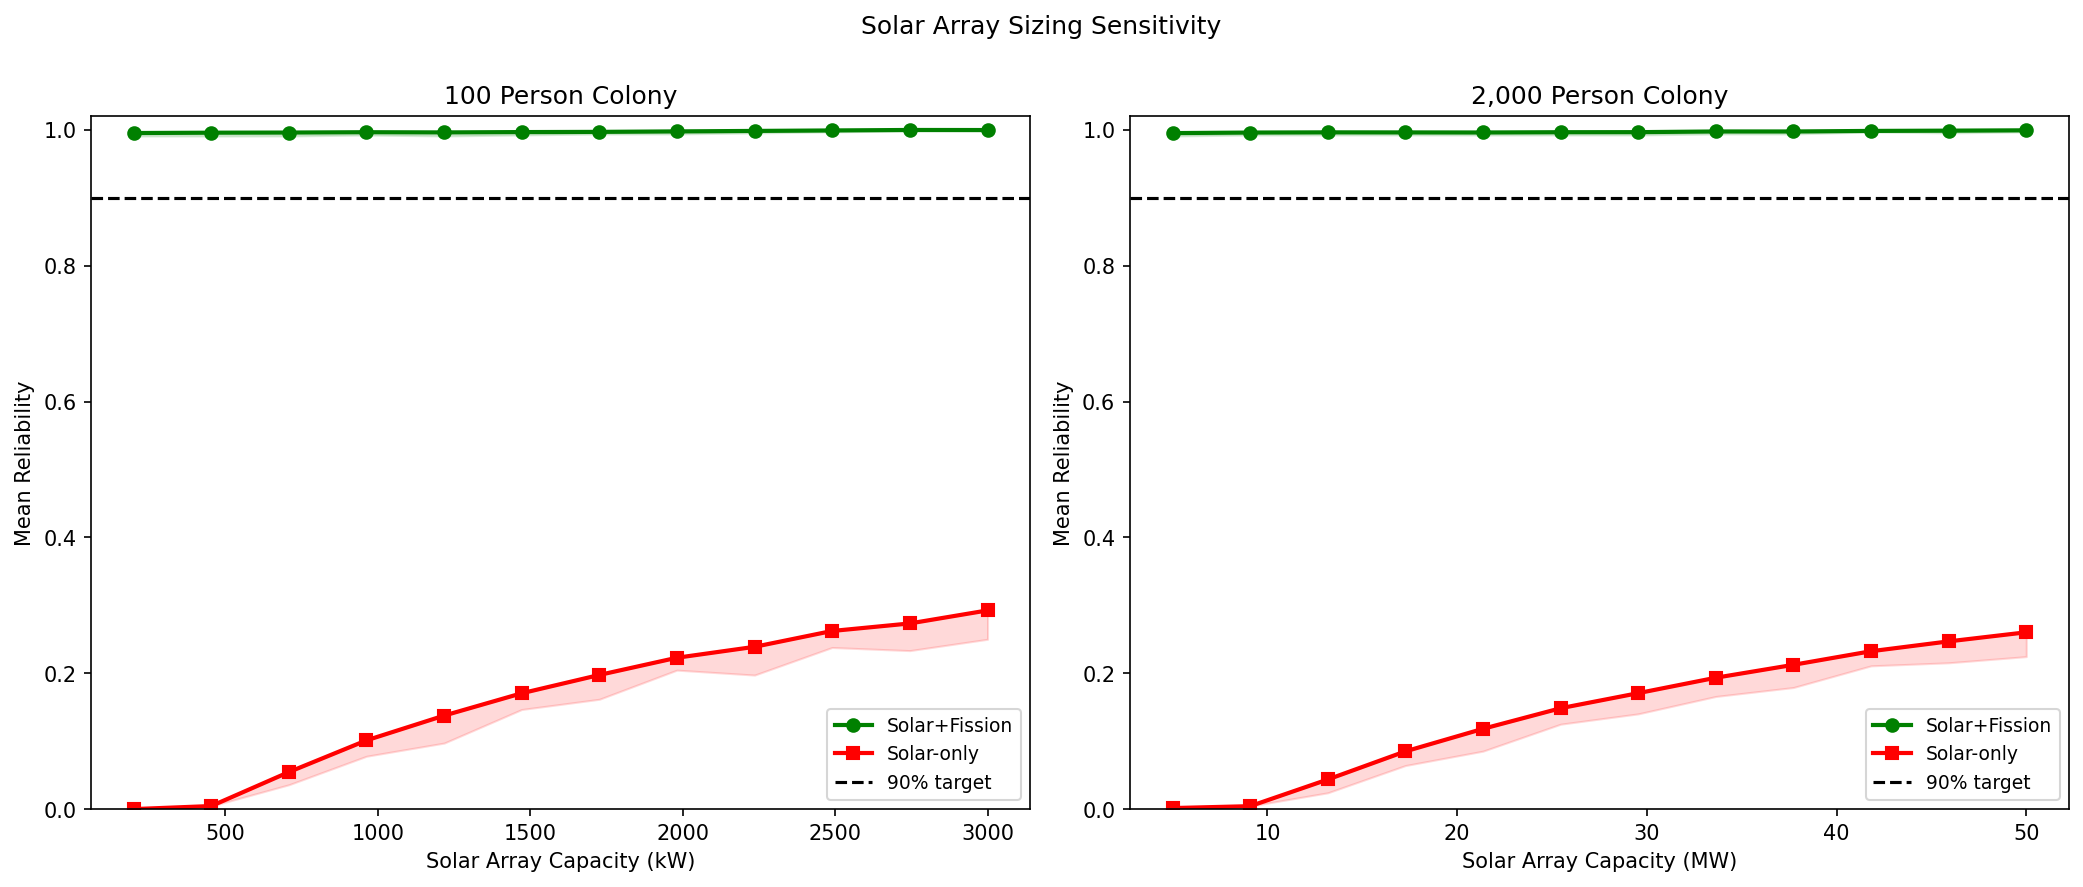
\includegraphics[width=\textwidth]{solar_sizing_sensitivity.png}
    \caption{Solar sizing sensitivity for larger colonies.}
\end{figure}

\begin{figure}[H]
    \centering
    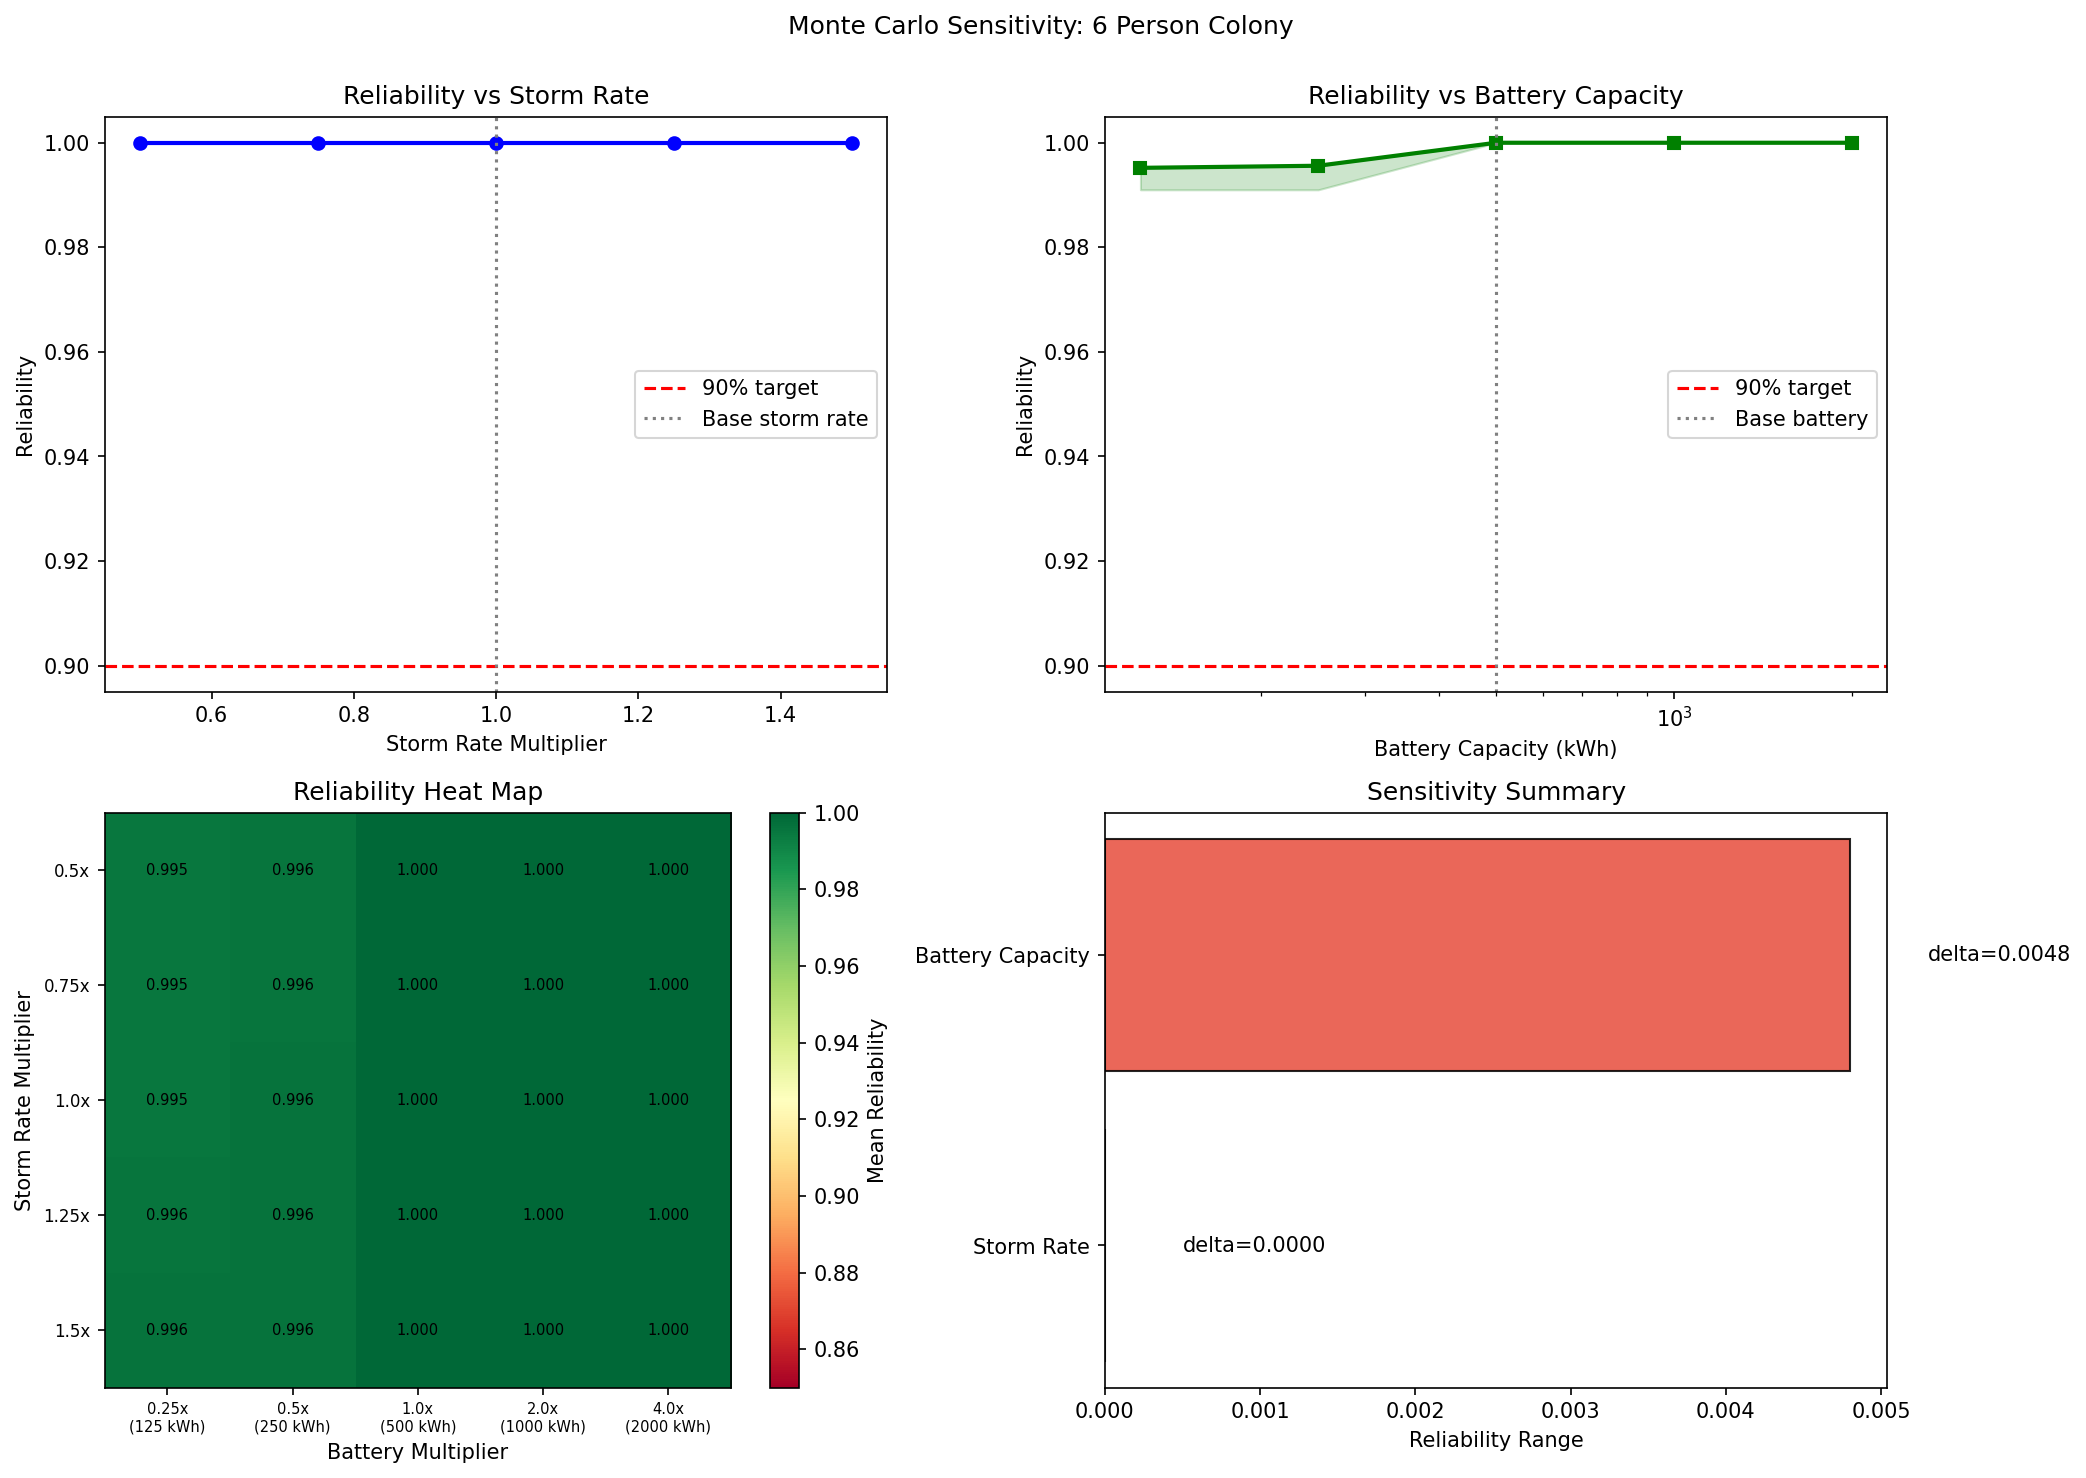
\includegraphics[width=\textwidth]{monte_carlo_sensitivity.png}
    \caption{Reliability sensitivity to storm rate and battery size in the 6 person baseline case.}
\end{figure}

\subsection{Forecast comparison}

The forecast comparison is secondary, but it is still internally consistent. The Transformer proxy gives the lowest error for all three colony sizes.

\begin{figure}[H]
    \centering
    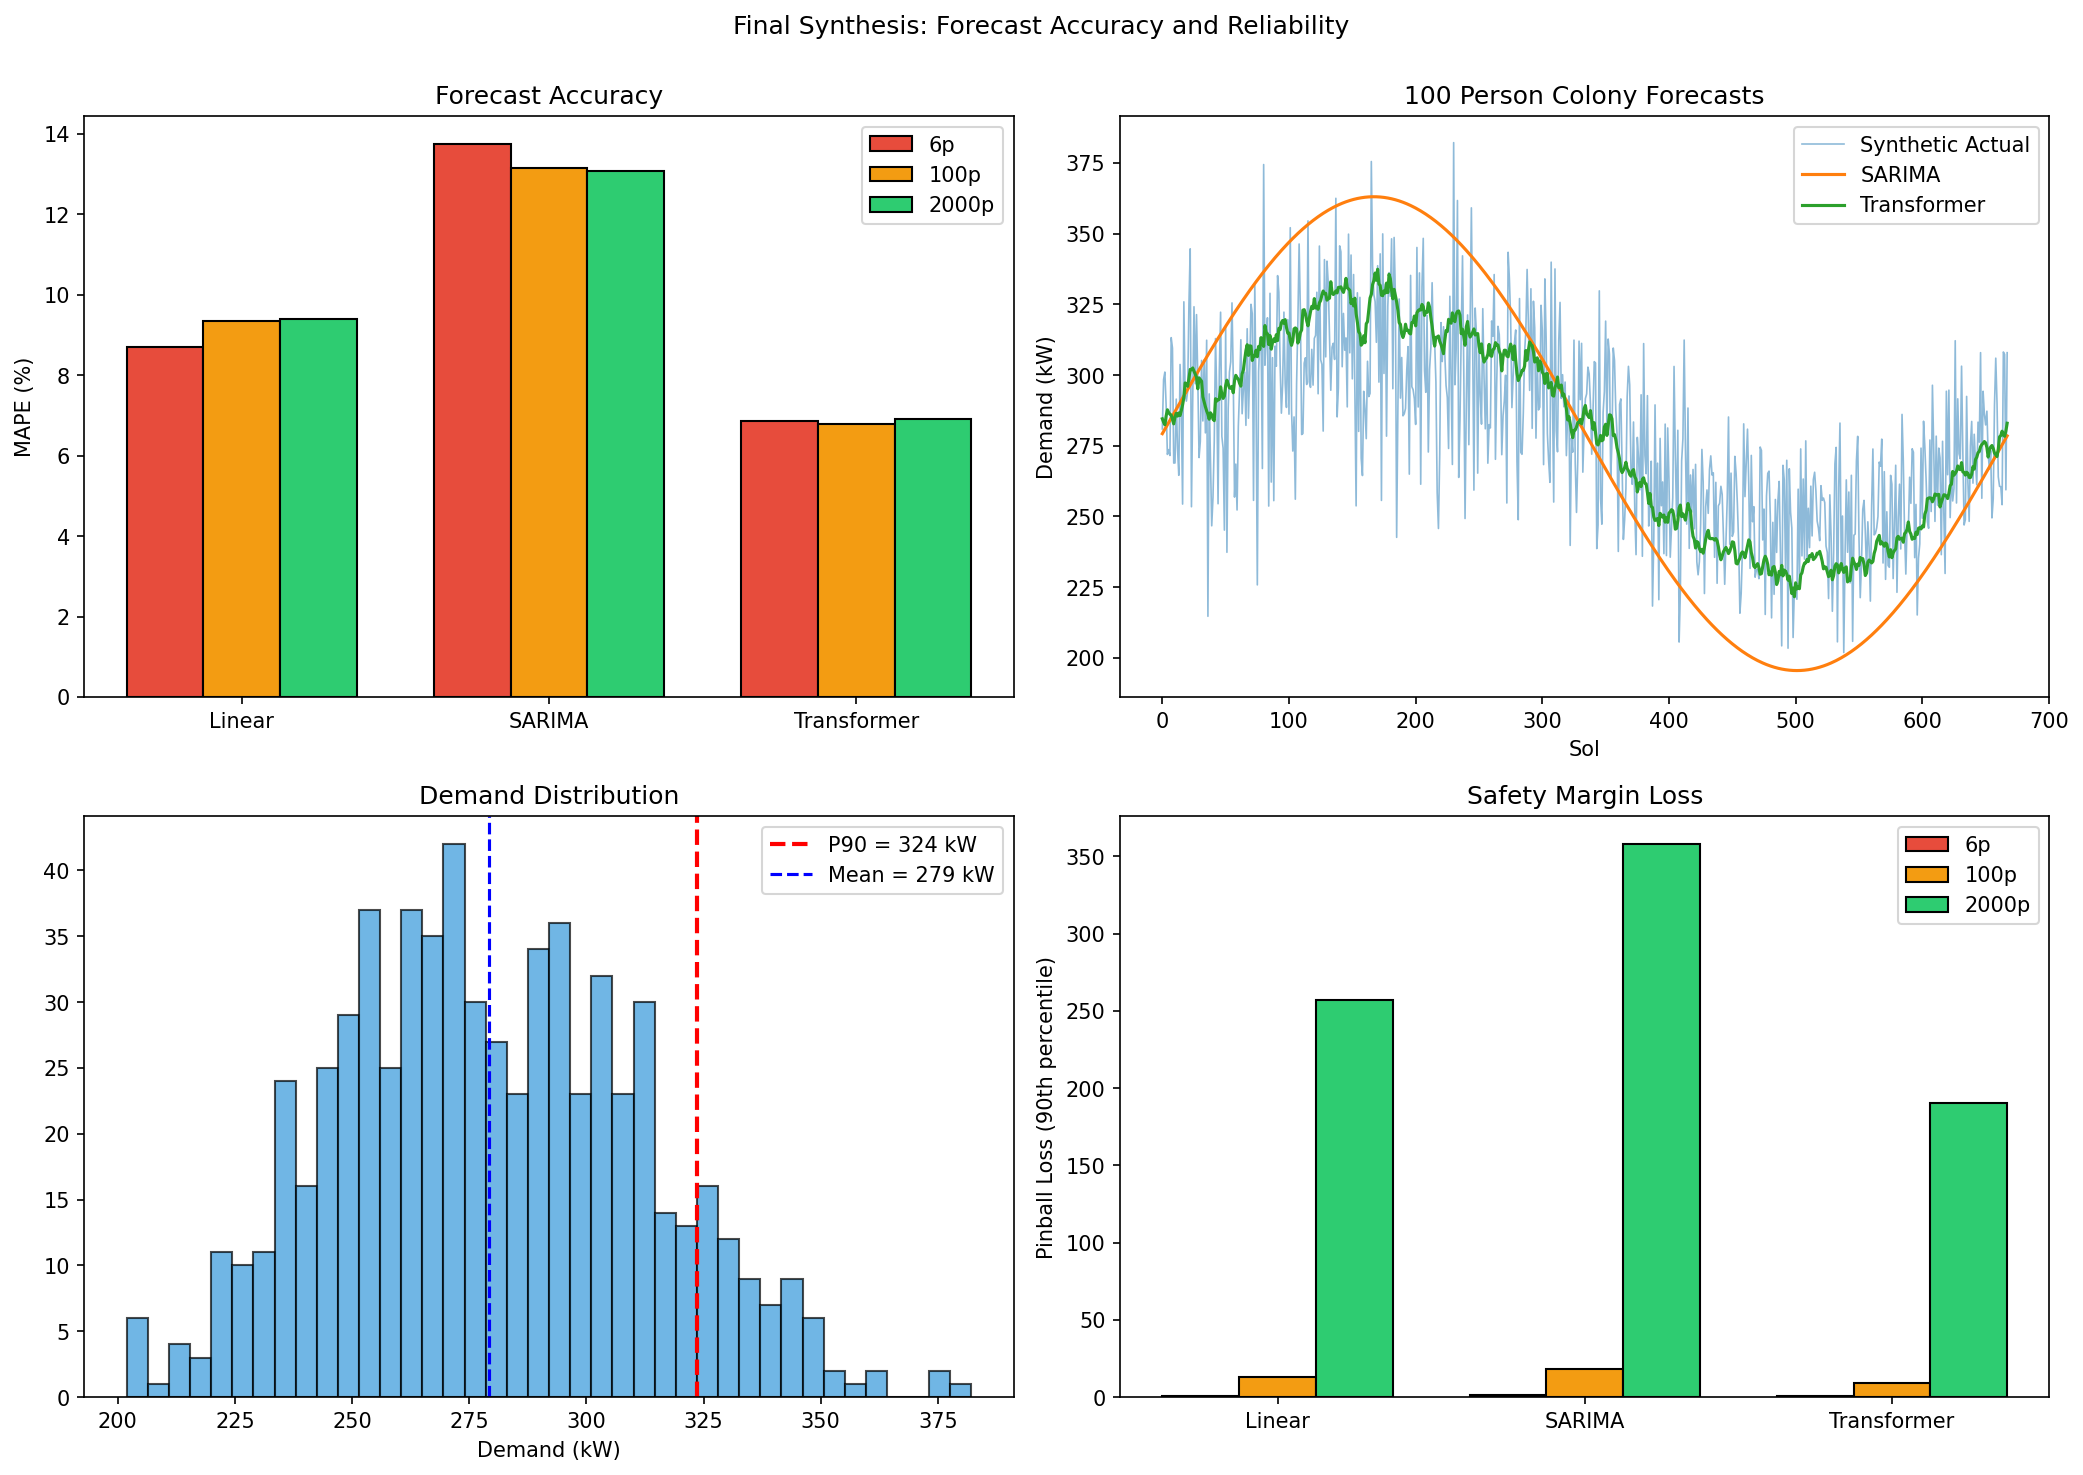
\includegraphics[width=\textwidth]{final_synthesis.png}
    \caption{Forecast comparison summary.}
\end{figure}

\section{Discussion}

The project supports a staged timeline for Mars colony energy rather than a one technology answer. The first stage is a small, early outpost. For that case, fission with solar support is the strongest answer in this repo. The reliability simulation shows that solar only systems fail badly under night and dust constraints, while solar plus fission reaches near full reliability for the 6 person baseline. This makes fission the practical early baseload source, with solar serving as useful supplemental generation rather than the backbone of the system.

The second stage is a growing settlement. At this point the colony can keep adding fission capacity and solar area, but the system starts to become a logistics problem. Solar remains attractive because panels are modular and can reduce fuel or reactor operating burden when conditions are good. The analysis does not support solar as the only supply, though, because dust storms and storage needs keep the reliability penalty high. In this middle stage, the most defensible architecture is still firm fission power, expanded solar, and enough storage to smooth short term variability.

The third stage is a large settlement where fusion becomes worth serious consideration. The fission scaling result is the main reason: reaching the same reliability threshold takes 8 Kilopower units for the 100 person case but 160 units for the 2{,}000 person case. That does not prove fusion is ready, and it does not make fission impossible, but it changes the planning question. At large colony scale, the mass, deployment, maintenance, and redundancy burden of many small fission units makes a high power fusion system more attractive if the technology matures. This is why the project treats fusion as a long run scale option rather than the first power source for Mars.

At the same time, the report should be clear about what is assumed rather than observed. The dust penalty curve is simplified. The habitat constants and storage tables are project inputs, not downloaded field datasets. Fusion performance numbers come from public concept descriptions, not operating reactors. Those limits do not erase the result, but they do set the right level of confidence.

\section{Reproducibility}

The project can be regenerated from the repo with:

\begin{center}
\path{.venv/bin/python run_analysis.py}
\end{center}

The input CSV source record is in:

\begin{center}
\path{docs/DATA_SOURCES.md}
\end{center}

The GitHub repository for the submitted project is:

\begin{center}
\href{https://github.com/vineet-reddy/MarsColonyNuclearFusion}{https://github.com/vineet-reddy/MarsColonyNuclearFusion}
\end{center}

\section{Conclusion}

This project does not argue that fusion is ready for Mars now. It argues for an energy timeline. A first Mars outpost should rely on fission with solar support because that is the only tested mix in the report that combines deployability with high dust storm reliability. A growing settlement should expand fission and solar together, using solar where it helps but not depending on it as the sole source. Once the colony grows beyond medium scale, fusion becomes worth planning for because the cost model and fission scaling study both point toward better long run scale economics if fusion technology matures. That staged conclusion is the result that stays stable across the classification work, the cost model, and the dust storm reliability analysis.

\begin{thebibliography}{9}

\bibitem{dra}
National Aeronautics and Space Administration.
\newblock \emph{Human Exploration of Mars Design Reference Architecture 5.0}.
\newblock NASA, 2010.

\bibitem{mdad}
J. M. Battalio and H. Wang.
\newblock \emph{The Mars Dust Activity Database}.
\newblock Icarus, 354, 2021.

\bibitem{eia}
U.S. Energy Information Administration.
\newblock \emph{Electric Power Annual, Table 4.08.B. Capacity Factors for Utility Scale Generators Primarily Using Non-Fossil Fuels}.

\bibitem{sparc}
A. J. Creely et al.
\newblock \emph{Overview of the SPARC tokamak}.
\newblock Journal of Plasma Physics, 86, 2020.

\bibitem{pss}
Princeton Satellite Systems.
\newblock \emph{Fusion Power for a Mission to Mars}.

\bibitem{avalanche}
Avalanche Energy.
\newblock \emph{Orbitron}.

\bibitem{moxie}
M. H. Hecht et al.
\newblock \emph{Mars Oxygen ISRU Experiment}.
\newblock Science Advances, 8, 2022.

\end{thebibliography}

\end{document}
